\subsection{using Deep Learning}
\subsubsection{Training}
\begin{figure}[H]
	\centering
	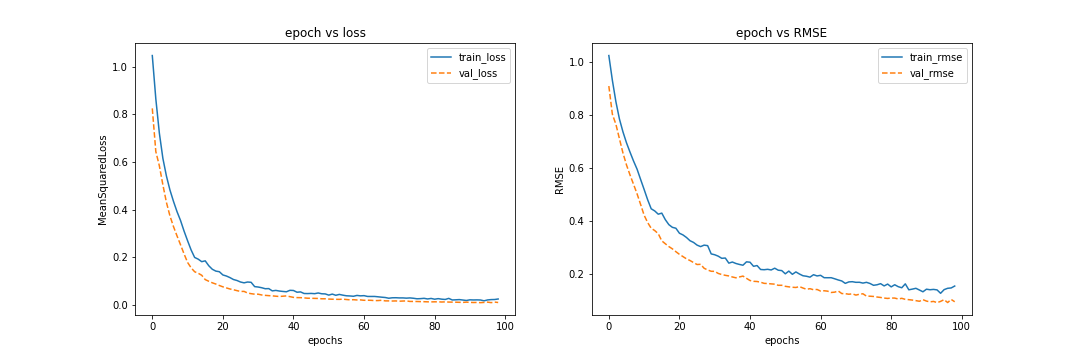
\includegraphics[width=\textwidth]{pantheon/lstm/05_epoch_vs_loss.png}
	\caption{Loss curve}
	\label{fig:loss_curve_union}
\end{figure}
\begin{figure}[H]
	\centering
	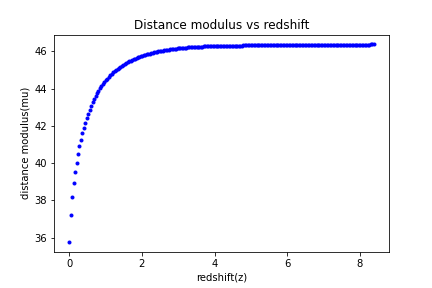
\includegraphics[width=0.8\textwidth]{pantheon/lstm/06_sample_reconstruction.png}
	\caption{Loss curve}
	\label{fig:reconstruction_lstm_union}
\end{figure}
\subsubsection{Testing redshift dependence of luminosity correlations}
\begin{table}[H]
\centering
\begin{tabular}{|c|c|c|c|c|c|c|c|c|}
\hline
Correlation & sample & N & a & $a_err$ & b & $b_err$ & $\sigma$ & $\sigma_{int}$\\
\hline
\multirow{3}{*}{$T_{lag}-L$} & low-z & 37 & 52.14 & 0.1 & -0.78 & 0.16 & 0.51 & 0.08\\
\cline{2-9}
 & high-z & 32 & 52.18 & 0.08 & -0.51 & 0.13 & 0.36 & 0.07\\
\cline{2-9}
 & All-z & 69 & 52.14 & 0.06 & -0.65 & 0.1 & 0.43 & 0.05\\
\hline
\multirow{3}{*}{$V-L$} & low-z & 47 & 52.14 & 0.25 & 0.65 & 0.37 & 0.92 & 0.14\\
\cline{2-9}
 & high-z & 57 & 52.56 & 0.24 & 0.1 & 0.23 & 0.66 & 0.07\\
\cline{2-9}
 & All-z & 104 & 52.33 & 0.14 & 0.32 & 0.15 & 0.79 & 0.07\\
\hline
\multirow{3}{*}{$E_{peak}-L$} & low-z & 50 & 51.92 & 0.09 & 1.46 & 0.18 & 0.6 & 0.07\\
\cline{2-9}
 & high-z & 66 & 52.0 & 0.06 & 0.99 & 0.16 & 0.4 & 0.05\\
\cline{2-9}
 & All-z & 116 & 51.95 & 0.05 & 1.28 & 0.12 & 0.5 & 0.04\\
\hline
\multirow{3}{*}{$E_{peak}-E_{\gamma}$} & low-z & 12 & 50.67 & 0.08 & 1.56 & 0.18 & 0.21 & 0.08\\
\cline{2-9}
 & high-z & 12 & 50.36 & 0.16 & 1.57 & 0.5 & 0.45 & 0.18\\
\cline{2-9}
 & All-z & 24 & 50.54 & 0.07 & 1.58 & 0.17 & 0.28 & 0.08\\
\hline
\multirow{3}{*}{$T_{RT}-L$} & low-z & 39 & 52.73 & 0.13 & -1.33 & 0.19 & 0.48 & 0.07\\
\cline{2-9}
 & high-z & 40 & 52.39 & 0.09 & -0.63 & 0.18 & 0.43 & 0.06\\
\cline{2-9}
 & All-z & 79 & 52.51 & 0.07 & -0.98 & 0.12 & 0.46 & 0.05\\
\hline
\multirow{3}{*}{$E_{peak}-E_{iso}$} & low-z & 40 & 52.6 & 0.1 & 1.6 & 0.2 & 0.59 & 0.08\\
\cline{2-9}
 & high-z & 61 & 52.51 & 0.07 & 1.13 & 0.17 & 0.47 & 0.05\\
\cline{2-9}
 & All-z & 101 & 52.53 & 0.06 & 1.36 & 0.13 & 0.52 & 0.04\\
\hline
\end{tabular}
\caption{A test caption}
\label{table_union_lstm}
\end{table}
\begin{figure}[H]
	\centering
	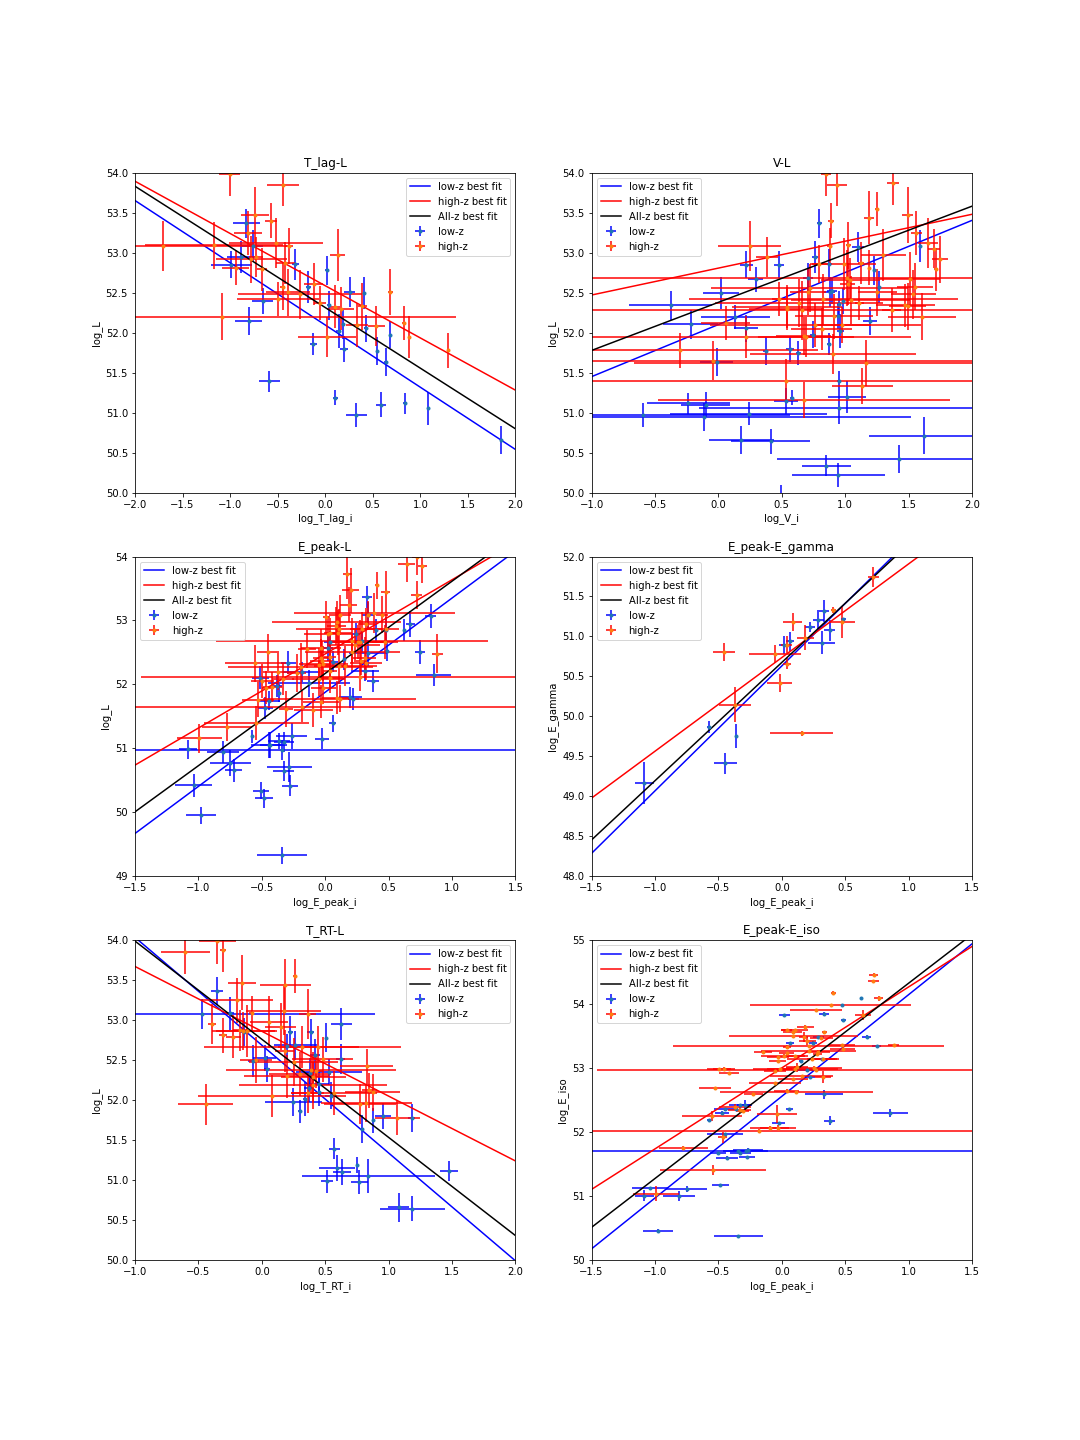
\includegraphics[width=\textwidth]{pantheon/lstm/15_correlatin.png}
	\caption{Luminsosity correlations best fit}
	\label{fig:correlation_lstm_union}
\end{figure}
\subsubsection{Calibrating distance modulus from $E_{peak}-E_{gamma}$ relation}
\begin{figure}[H]
	\centering
	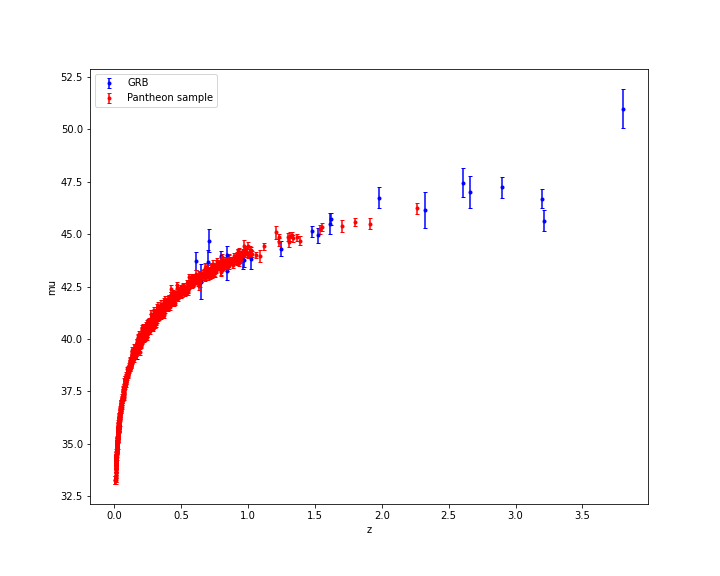
\includegraphics[width=0.7\textwidth]{pantheon/lstm/16_GRB_reconstruction.png}
	\caption{GRB Hubble Diagram}
	\label{fig:HD_GRB_LSTM_union}
\end{figure}
\subsubsection{Constraints on dark energy}
\begin{figure}[H]
	\centering
	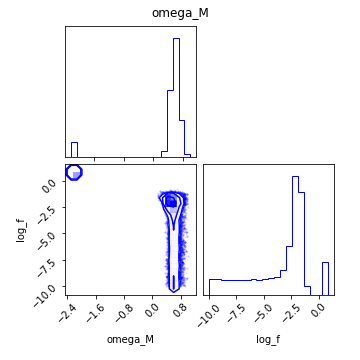
\includegraphics[width=0.5\textwidth]{union/lstm/18_omega_M_corner_plot.png}
	\caption{GRB Hubble Diagram}
	\label{fig:OmegaM_lstm_union}
\end{figure}